\documentclass[a4paper,doc,natbib]{apa6}

\usepackage[english]{babel}
\usepackage[utf8x]{inputenc}
\usepackage{amsmath}
\usepackage{graphicx}
\usepackage[colorinlistoftodos]{todonotes}
\usepackage{enumitem} % Customized lists
\usepackage{float}
\usepackage{hyperref}
\usepackage{subcaption}
\setlist[itemize]{noitemsep} % Make itemize lists more compact

\title{Realistic analytic variability in fMRI:\\The problem and a potential solution}
\shorttitle{Realistic analytic variability in fMRI}
\author{Kendra Oudyk}
\affiliation{\\ Final project for NEUR608 Neuroimaging Data Science \\ Drs. Boris Bernhardt and Bratislav Misic, Instructors \\ McGill University \\ 2019-12-10}

\abstract{There has been concern recently over reproducibility issues in neuroimaging. These issues are partially due to analytic variability; results may change when different choices are made for analyzing the data. The purpose of this study is to investigate the effect of research group on fMRI results with a more realistic estimate of analytic variability, as well as to explore a potential solution. Here, we show that, in a realistic setting where 55 separate research teams analyze the same data, there is variety in the analysis choices and in the group-level results. Partial least squares (PLS) revealed that the analysis choices are related to the group-level results. The more important analysis choices were whether the team used the fmriprep-preprocessed data, the size of their smoothing kernel, and whether they used randomise to produce their statistical images (in FSL). A closer look at the differences in analytic range between those who do and do not use the fmriprep data reveals a spatial bias, and suggests that preprocessing is an important source of analytic variability. We also explored the use of the consensus result across analysis teams as a way to improve the accuracy of results. To this end, we used the results of an automated meta-analysis of the relevant literature, generated using NeuroQuery \citealp{dockes2018text}, as an approximate ground truth. The consensus result did not strongly resemble the NeuroQuery results, and the consensus did not have greater resemblance than the group-level maps. However, there are a number of limitations should be addressed before concluding that taking the consensus result across different methodological pipelines is not useful in the face of analytic variability. These results have implications for our understanding of the stability of fMRI results across teams.}

\begin{document}
\maketitle

Keywords: Reproducibility, fMRI, meta-analysis, decision-making, NARPS.

\vspace{1cm}

\section{Introduction}
Over the past few decades, researchers have become more aware of reproducibility issues in science \citep{ioannidis2005most}. In order for a result to be accepted as scientific knowledge, the result needs to be reliable. It should be reproduced when the study is performed multiple times with the exact same methods, and it should be stable over small differences in methodology. Yet, we are becoming more aware that seemingly minor methodological choices can influence results. 

There has been concern over these reproducibility problems in functional magnetic resonance imaging (fMRI). There are many steps involved in preprocessing and analyzing fMRI data, with different options for how to perform each step, as well as different software that implement the same method. A researcher must make methodological choices in the absence of a clear `correct' choice. These researcher degrees of freedom are often under-reported \citep{carp_secret_2012}, and can influence results \citep{poldrack2017scanning, carp_plurality_2012}. Even some broadly accepted methods, such as cluster-wise inference, have been shown to be problematic in some software implementations; this is especially worrisome because the increased false-positive results may be distributed in non-uniform manner over the brain \citep{eklund_cluster_2016}. Further, some variables that do not seem like explicit choices can make a difference; results can vary over different versions of the same software \citealp{gronenschild_effects_2012} and different computer operating systems (e.g., Macintosh versus Windows; \citealp{glatard_reproducibility_2015}). Thus, it is clear that these methodological choices have an impact on results, calling into question the reliability of the results and the accuracy of the knowledge derived from the results. 

However, we do not yet know how severe these effects are in realistic situations. Previous studies have systematically evaluated the role certain methodological variables, but it is not clear what would be the variation in results across real analysis teams. It is also not entirely clear how we can overcome these reliability issues. The goals of this study are to investigate the effect of research group on fMRI results in a realistic situation, as well as to explore a potential solution.

To this end, we will look at the results obtained by different research teams who analyzed the same data using their regular pipelines \citep{botvinik-nezer_fmri_2019}. The data given to the analysis teams was from a study of decision-making under risk, using the mixed-gambles task \cite{tom_neural_2007}. The analysis teams were given instructions on which hypotheses to test, and which analyses to perform (see \citealp{botvinik-nezer_fmri_2019} for details). The teams were given the option of either using data that was already pre-processed with fmriprep \citep{esteban2019fmriprep} or preprocessing the data themselves. Then they were supposed to perform the remaining analyses using their lab's standard methods, and return the group-level results maps as well as a log of the methods they used. 

In the present study, we use these various group-level results in order to investigate the role of analysis team in fMRI results, and to explore a potential solution to this analytic variability in fMRI. This will be done in two stages: first, we sill describe the problem of how results can vary over analysis teams; then, we will explore whether a potential solution is to use the consensus result across teams. 

\section{Methods} \label{sec:methods}

\subsection{Acquisition and preprocessing of the participant-level data}
\subsubsection{Participants}
There were 119 healthy participants in the original study. Each participated in one of two conditions, with 60 in the equal-indifference condition and 59 in the equal-range condition (described below) After excluding participants according to the preregistered exclusion criteria, there were 108 participants, with 54 in the equal-indifference condition (all right-handed, 30 females, mean age = 26.06 $\pm$ 3.02), and 54 in the equal-range condition (all right-handed, 30 females, mean age = 25.04 $\pm$ 3.99). The exclusion criteria can be found at \url{https://aspredicted.org/ru8ua.pdf}, and the specific numbers of participants excluded for different criteria can be found in \cite{botvinik-nezer_fmri_2019}, the data report for the original participant-level dataset. No participants reported a history of psychiatric or neurological disorders.

\subsubsection{Procedure}
Participants gave written consent to participate when they arrived at the lab. Then they received 20 ILS cash for participating, and were told that they would receive the remaining 100 ILS following the experiment. Then the experimenter explained how to behave in the scanner, and the participant did a test-run of the behavioral task outside the scanner and confirmed that they understood the task. Next, in the scanner, the participants performed their behavioral task in four runs of fMRI scanning. This was followed by field mapping and anatomical scans with no task. There was additional data that was collected but not used in the present study; see \cite{botvinik-nezer_fmri_2019} for details. At the end, one of the gambles that the participant accepted during the mixed gambles task was chosen at random and played. 

\subsubsection{Task} \label{sec:task}
The behavioral task was the mixed-gambles task. There were four runs, each containing 64 trials and lasting 543 seconds (543 volumes). In each trial, the participant was presented with a mixed gamble in the form of a potential gain alongside a potential loss. They were given up to 4 seconds to indicate whether to take the gamble, using button presses with their right hand. After they responded or 4 seconds had passed without a response, they were presented with a grey screen until the next gamble was presented. The total inter-trial interval, including the response time and the grey screen, ranged from 5.0 to 9.9 seconds (mean 6.94). Participants were not aware of the success or failure of their gambles during scanning. See Figure \ref{fig:task} for an illustration of the task in these two conditions. 

The two conditions differed in the ratio of potential gains to losses, that is, the level of risk. In the  Equal Range condition, the range of potential gains was equal to the range of potential losses. In the Equal Indifference condition, the range of potential gains was twice the range of potential losses. This is called `equal indifference' because of the theory that people need the the potential gain to be twice the amount of the potential loss in order to consider it a fair risk. 


\begin{figure}[!htb]
    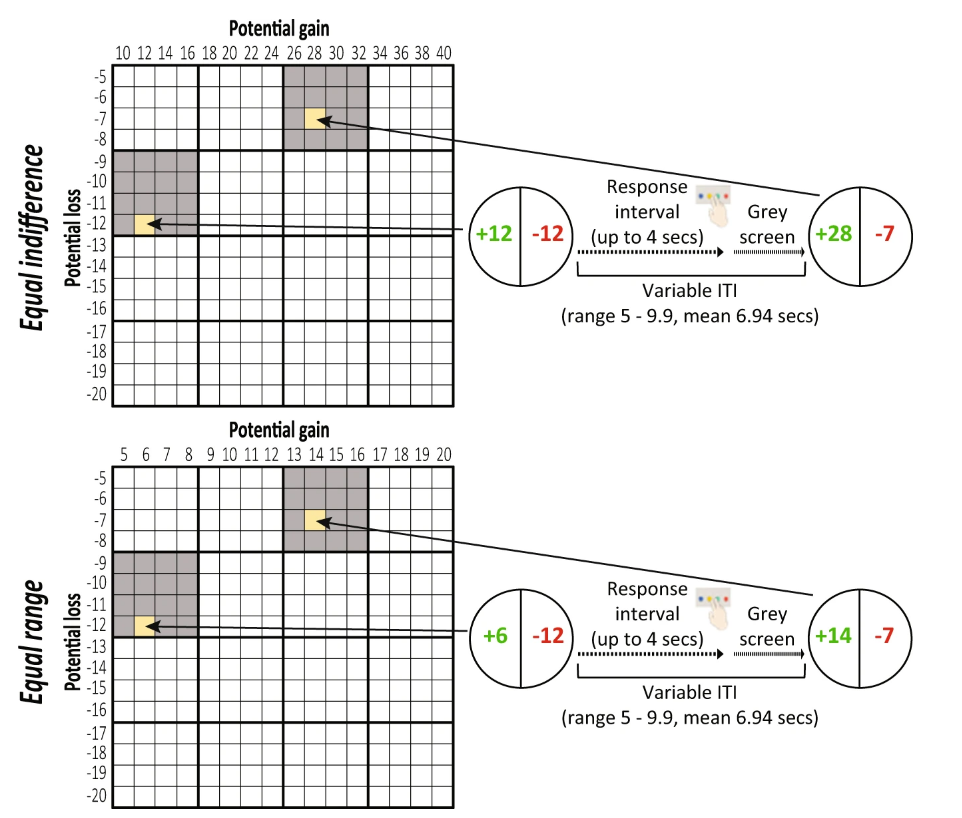
\includegraphics[width=\textwidth]{figures/botvinik-nezer_fig1.png}\vspace{.5cm}
    \caption{\label{fig:task} This figure illustrating the behavioral task was taken from \cite{botvinik-nezer_fmri_2019}. This is their caption: ``An illustration of the mixed gambles task design. Adapted from \cite{tom_neural_2007}. During each trial, the participant was presented with prospects including the potential gain and loss, until a response was made or four seconds passed. The next gamble was presented following a jittered inter-trial interval (ITI). Potential gains and losses were sampled from the presented gain/loss matrices, which were different for the equal indifference and equal range conditions. The amounts of money are in ILS.''}
\end{figure}

\subsection{Analysis of original data}
The Neuroimaging Analysis Replication and Prediction Study (NARPS) was advertised and research teams could apply to analyze the data. In return, a maximum of three researchers from each team could be co-authors on the resulting papers.

Seventy teams were given access to the data in November 2018, and were allowed 3 months to perform a whole-brain corrected analysis of task-related activation for each hypothesis. These hypotheses were selected based on past results on this topic, and are described in \cite{botvinik-nezer_fmri_2019}. The teams were told to use their standard analysis pipeline, and they had the option of using the raw or preprocessed data (preprocessed using fmriprep CITE). 

At the end of the analysis period, each team returned the following results:
\begin{itemize}
	\item A description of how they analyzed the data,
	\item A yes/no decision for each of the nine hypotheses, 
	\item A group-level thresholded statistical map for each contrast, 
	\item A group-level unthresholded statistical map for each contrast, and
	\item If available, participant-level contrast maps and variance maps. 
\end{itemize}

\subsection{Data used for the present study}
The results from 15 analysis teams were rejected due to poor resampling to the template brain (3), missing thresholded images (1), using a surface-based analysis (2), not submitting unthresholded images (1), using small-volume correction (2),  poor normalization (1), and missing data (3). These decisions were made before we received the data. Thus, our dataset consisted of the group-level maps and pipeline summaries from 55 analysis teams. 

The data for this study consisted of the results map from each analysis team, for two of the hypotheses. These are group-level whole-brain unthresholded statistical maps (z-maps). Team identity was anonymized before we received the data. Both hypotheses were meant to investigate a parametric effect of gain (winning a gamble) in the ventromedial prefrontal cortex, the first hypothesis investigating this effect in the equal-indifference condition, and the second in the equal-range condition. We first examined the set of group-level maps from the first hypothesis. Then we attempted to replicate these results in the set of maps from the second hypothesis. 

It should be noted that these hypothesis target the ventromedial prefrontal cortex, but this regional specification is not of interest in the present study. The analysis teams returned whole-brain group maps and we performed whole-brain analyses on these maps. 

\subsection{Analysis summary}
The analyses can be broadly divided into three stages:
\begin{enumerate}
\item First, we will describe the problem: how analyses impact results. To this end, we will highlight the differences in pipeline choices and visualize the range in results to get an idea of how much variation is present in the methods and results from different analysis teams. Further, in order to explore which methodological choices introduce the most variance across teams, we will use partial least squares (PLS; \citealp{mcintosh2013multivariate, mcintosh2004partial}) to associate methodological choices with the group-level maps from each analysis team. 
\item Second, we will explore a potential solution: using the consensus result across analysis teams. We will calculate this consensus result by meta-analyzing the group-level maps from the various analysis teams. Then we will evaluate whether this consensus result is closer to the findings in the literature, compared to the individual group-level maps. To this end, we will perform an online meta-analysis of papers on the topic covered in this dataset, and then compare this literature meta-analysis result with a) our consensus result, and b) the individual group-level maps. The assumption here is that the meta-analytic result can be taken as a more `accurate' result on this topic, since it it represents the consensus across many studies. According to the NeuroQuery web interface, the number of papers in this meta-analysis appears to be 329,956, since that is the sum of the number of papers found for each term. However, knowing that the database contains approximately 14,000 papers, it seems likely that there is overlap in papers between these terms
\item Finally, we estimate the reliability of these results by replicating the above analysis using the NARPS data for the second hypothesis. The above analysis were performed on the data from the first hypothesis. These hypotheses are the same, but are tested on different samples of participants, who underwent slightly different conditions (see the task description for details).
\end{enumerate}

\subsection{Analyses I: The problem variability across teams}
Here, we describe the variation in analysis choices across analysis teams, and associate this variance with variance in the results across teams. 

\subsubsection{Summary of the analytic variability}
In order to look at the variation in analysis choices across teams, we selected four analysis choices that were suitable for quantification because they were numerical or easy to categorize and code into dummy variables. These variables were 1) whether the teams used the fmriprep-preprocessed data, 2) the size of their smoothing kernel, 3) the analysis software, and 4) the significance-testing method. The distributions of choices for each of these variables were visualized in histograms.

Following the method of \cite{carp_plurality_2012} when he showed his results after running multiple pipelines on the same data, we calculated the mean activation and the analytic range of the group-level maps from the analysis teams. These were respectively calculated as the mean and the range of z-scores across teams, for each voxel. 

\subsubsection{Associating analysis choices with results using partial least squares (PLS)}
In order to explore which analysis choices may have had the greatest impact on results, we used partial least squares (PLS \citealp{mcintosh2013multivariate, mcintosh2004partial}) to associate these pipelines-choice variables with the group-level results. PLS is a multivariate associative technique that is a form of reduced-rank linear regression in the same family of techniques as canonical correlation. Its goal is to find linear combinations of two sets of variables (here, analysis choices and brain data) that best explain their combined variation. These linear combinations are the new `dimensions' found in the data. 

To perform PLS, we first standardized the brain data and scaled all analysis-choice variables between 0 and 1 (they could not be standardized because they were ordinal/categorical). We then took the cross-correlation of these two sets of variables using Spearman's correlation. Specifically, these two sets are 1) a \textit{g}-by-\textit{k} matrix of group-level maps with \textit{k} voxels for each of the \textit{p} analysis teams; and 2) a \textit{g}-by-\textit{p} matrix of \textit{g} methodological choices for each analysis team.  Next, we use singular value decomposition to decompose this correlation matrix into two singular matrices, one for each set of multivariate data, as well as a set of singular values. This process is illustrated in Figure \ref{fig:pls_ill}. 

Regarding the interpretation of the results of this type of decomposition, the rows of each singular matrix correspond to the columns of their respective set of variables on either side of the original correlation. The columns of the singular matrices represent the new dimensions that were found to contain the most variance in the correlation matrix. In these dimensions, the correlation between the two sets of variables is maximized. The singular value for each dimension describes how well the dimension captures the variance in the original data. 

\begin{figure}[!htb]
    \centering
    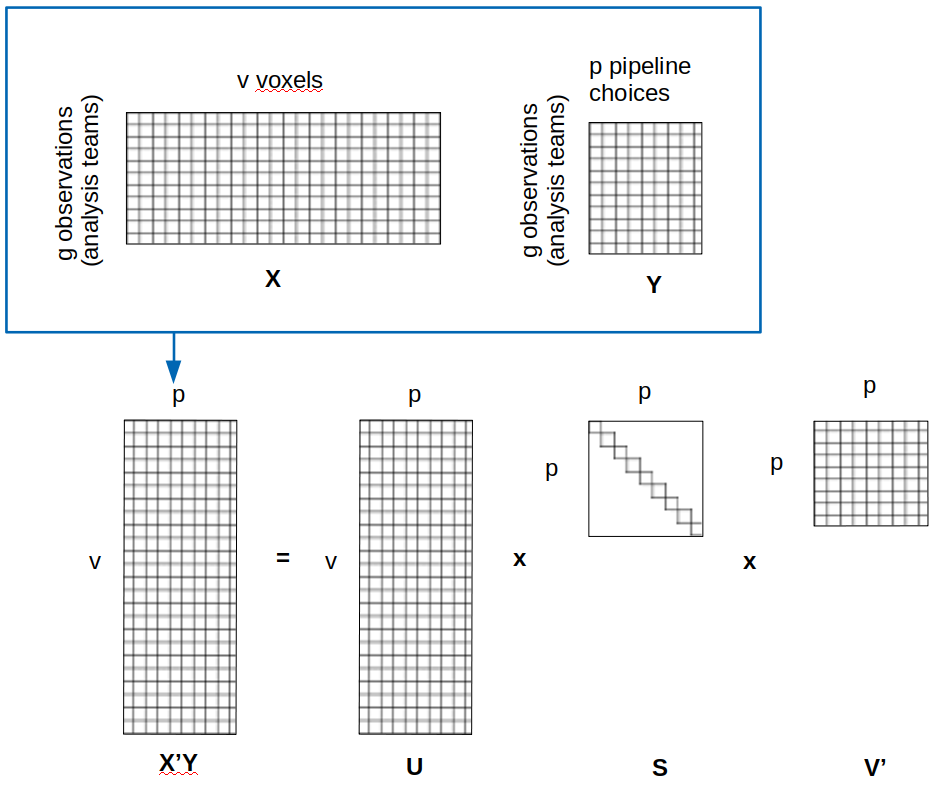
\includegraphics[width=\textwidth]{figures/pls_illustration.png}
    \caption{Illustration of PLS in this use case}
    \label{fig:pls_ill}
\end{figure}

\subsubsection{Selecting useful components}

In order to choose components that are useful for explaining our data, we can look at how much variance in the original correlation matrix is explained by the components, as well as the significance of the amount of variance explained. 

We calculated the variance explained in each dimension by taking the square of a given dimension's singular value, divided by the sum of all the squared singular values. 

To test whether the components had values greater than would be expected by chance, we performed non-parametric significance testing \citep{mirchi2018tracking, nichols2002nonparametric}. We permuted the rows of the matrix of analysis-choice variables 1000 times. For each permutation, we redid the PLS and used Procrustes rotation to align the singular matrix for the analysis choices with the corresponding original singular matrix (from the unpermuted data). We then calculated the singular values in this new space, where permutation had destroyed the relationship between the two sets of variables, and the rotation aligned the singular values so that a null distribution could be built for each component. To derive a \textit{p}-value for each component, we calculated, for each singular value, the proportion of singular values in these null distribution that were higher than the original singular value.


\subsection{Analyses II: Exploring the consensus result as a potential solution}
\subsubsection{Meta-analysis of NARPS group-level maps} 

We meta-analyzed these group-level z-maps using a fixed-effects model. We did not have access to the group-level standard-error maps from the analysis teams, or else we could have done a mixed-effects model, which considers the fact that the analysis teams were a sample from all possible analysis teams, and which is considered the gold standard in neuroimaging meta-analysis \citep{salimi-khorshidi_meta-analysis_2009}. In this study, this model is estimated in a mass univariate manner, in three levels using summary statistics between levels. Here, we briefly describe each level. 

At the first level, the BOLD signal in each voxel is modelled using a linear combination of time series that describe the task structure. This can be expressed as $ Y_{i}=X_{i} \beta_{i} + \epsilon_{i}$, where \textit{Y\textsubscript{i}} is a \textit{n}-by-1 vector of the preprocessed BOLD signal over \textit{n} observations (i.e., scans) for the given participant \textit{i}; \textit{X\textsubscript{i}} is a \textit{n}-by-\textit{p} matrix with \textit{p} regressors that describe the time course of events that occurred during scanning; \textit{$\beta_i$} is a \textit{p}-by-1 vector of the parameter weight for each of the \textit{p} stimulus regressors; and \textit{$\epsilon_i$} is a \textit{n}-by-1 vector of a within-subjects residual. This is a fixed-effects model because the observations (i.e., scans) are not sampled from a larger population. 

At the second level, the level-1 parameter weights (or the contrast between sets of parameter weights) is modelled as a constant over participants, essentially modelling where the mean activation from level 1 is not equal to zero. This is the equivalent of a one-sample t-test. For generalization beyond the sample of participants, this should be a random-effects model because observations (i.e., participants) are randomly sampled from a larger population. Together with the first-level analysis, this is a mixed-effects model (combining fixed and random effects). The test of the mean at the second level becomes a test of the weighted mean, the weights being the level-1 variance for each participant (i.e., SSE\textsubscript{w}, the sum of $\epsilon_{i}^2$, or the sum of squared errors within participants). This level can be expressed as $\beta_{j}=Z_{j} \alpha_{j} +\delta_{j}$, where $\beta_j$ is a \textit{N}-by-1 vector of the level-1 (possibly contrasted) parameter estimates over \textit{N} observations (i.e., participants) for the given analysis team \textit{j}; \textit{Z\textsubscript{j}} is a \textit{N}-by-1 vector of the SSE\textsubscript{w} for each of the \textit{N} participants, modelling the weighted group mean (in practice, the assumption is often made that the SSE is equal for all participants, so this becomes a vector of ones); \textit{$\alpha_j$} is a scalar that is the parameter weight for the single regressor; and \textit{$\delta_j$} is a \textit{N}-by-1 vector of the between-subjects residual. The first two levels were performed by the analysis teams. 

At the third level, the level-2 parameter weights for each team is modelled in the same way as the level-3 parameter weights. This level can be expressed as $\alpha=V \gamma +\zeta$, where $\alpha$ is a \textit{g}-by-1 vector of the level-2 parameter estimates over \textit{g} observations (i.e., analysis teams); \textit{V} is a \textit{g}-by-1 vector of the SSE\textsubscript{b} for each of the \textit{g} teams, modelling the weighted group mean; \textit{$\gamma$} is a scalar that is the parameter weight for the SSE\textsubscript{b} regressor; and \textit{$\zeta$} is a \textit{g}-by-1 vector of the between-subjects residual. The result of this final level (i.e., the meta-analysis) is a map with a parameter weight for each voxel, which were converted into t-statistics by dividing the weights by the standard error. This t-map is the consensus result across analysis teams. 

\subsubsection{NeuroQuery meta-analysis of relevant literature}

In order to compare these results against the literature, we compared our meta-analytic results with results of a meta-analysis of previous fMRI activation studies on this topic. To this end, we used an automated term-based meta-analytic, searching for ``Loss aversion in decision-making under risk'', which is part of the title of the original paper by \cite{tom_neural_2007} on this topic that was published in \textit{Science}: ``The Neural Basis of Loss Aversion in Decision-Making Under Risk''.

The meta-analytic tool that we used NeuroQuery (\citealp{dockes2018text}, \url{https://neuroquery.saclay.inria.fr/}). The original automated online meta-analytic tool was NeuroSynth (\citealp{yarkoni2011large}, \url{https://www.neurosynth.org/}). However, its search functionality is different and was less suitable for the paradigm in this study. While NeuroSynth takes searches for specific single and compound words that are common in the fMRI literature, NeuroQuery can take more complicated searches, like full sentences. It uses a predictive modelling approach to finding relevant papers by expanding the original search terms using synonyms.

The data used by this tool is word frequencies in publication texts, so the topic labelling may not be ideal. Further, it only has access to the peak coordinates that are reported in papers, so they can only perform coordinate-based meta analyses. Image-based meta-analyses are preferable, since they contain more information that is lost in thresholding and peak extraction. However, the strength of this type of tool lies in the large number of studies that can be assessed.

\subsubsection{The usefulness of meta-analysis across analysis teams}

Taking the consensus result across analysis teams may be useful for addressing the problem of analytic variability in fMRI. If a result is stable over variation in methodological choices made by analysis teams, this is promising for the reliability of the result. This stable result would be present in a meta-analysis across teams. 

However, one could still question whether this consensus result is more accurate. It is not possible to explicitly test accuracy of the consensus result without the ground truth, the known true result, to use as a comparison. But it could be argued that the closest we can get to a `true' neuroimaging result in humans using non-invasive methods is to look at the consensus result across many past neuroimaging studies on the same topic. 

Thus, in order to evaluate whether the consensus result across teams was `accurate' in terms of similarity to past findings, we performed a Spearman's correlation between the online meta-analytic result from past studies with the consensus result across NARPS analysis teams.

We tested the null hypothesis of no relationship between the two maps using a standard parametric test, but we also performed non-parametric significance testing in the form of a spin test \citep{alexander2018testing} in order to account for the spatial autocorrelation that is present in brain data, using Brain Space \citep{de2019brainspace}. This test requires the data to be in surface space rather than volume space, so we performed both the correlation and significance testing in surface space. 

In this case, the spin test works by projecting one of the maps onto a sphere, rotating the sphere, and recalculating the correlation between the two maps. This type of permutation was done 1000 times to build a distribution of null correlation coefficients. Then, we found the percentile of the correlation coefficient between the non-permuted maps (i.e., the real correlation). This percentile, subtracted from 1, is the non-parametric \textit{p}-value, or the probability of getting a result this size if the null hypothesis of no correlation is true.

Next, in order to determine whether the consensus result is better than the results from individual teams, we used Spearman's correlations to perform pairwise comparisons of the online meta-analytic result from the literature with a) the meta-analytic result across NARPS analysis teams, and b) the individual group-level maps from each team. We then examined the distribution of these correlation coefficients.

\subsection{Analyses III: Replication}
In order to evaluate the reliability of our results, we performed all of the above analysis on the data from the second hypothesis in the NARPS study. The above analysis were performed on the data from the first hypothesis, which tested the same effect in a different condition, with a different sample of participants (see the task description in the Methods section for details). 

\section{Results}
\subsection{Results I: The problem variability across teams}

\subsubsection{Summary of the analytic variability}
In Figure \ref{fig:1Amaps}, one can see the mean activation and the analytic range (of $z$-scores) across the analysis teams' group-level maps. This follows the visualization method of \cite{carp_plurality_2012} for displaying his results when he used many analysis pipelines on the same dataset. However, in this case, we see what could be a more realistic description of the analytic variability across real research teams using their usual analysis methods, assuming that these teams used a sampling of analysis choices that well-represents the field. 

\begin{figure}[!htb]
	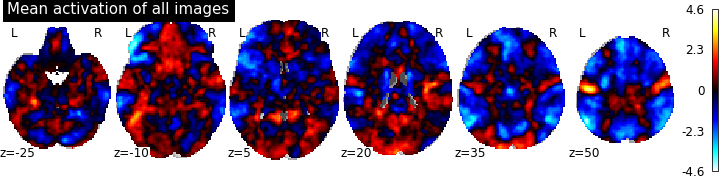
\includegraphics[width=\textwidth]
	{figures/results1B_hypo1_Mean-activation-of-all-images.png}
	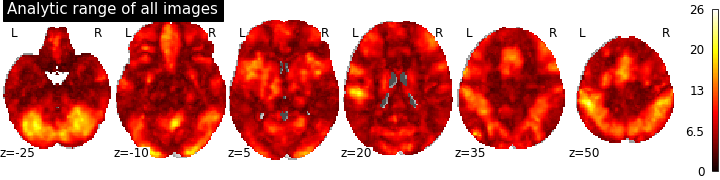
\includegraphics[width=\textwidth]
	{figures/results1B_hypo1_Analytic-range-of-all-images.png}
	\caption{\label{fig:1Amaps} Mean activation ($z$-scores) and analytic range ($z$-scores) of all the NARPS group-level maps.}
\end{figure}

\begin{figure}[!htb]
	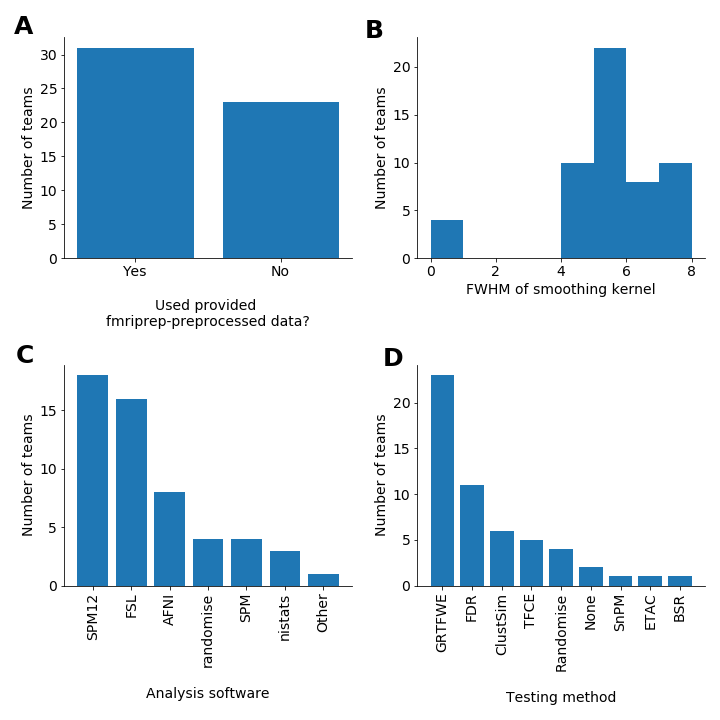
\includegraphics[width=\textwidth]
	{figures/result1A_methods_histograms.png}
	\caption{\label{fig:1Ahists} The distribution of analysis choices for A) whether the fmriprep-preprocessed data was used, B) the size of the smoothing kernel used in preprocessing, C) the software used to analyze the data, and D) the method that was used for hypothesis testing.}
\end{figure}

The analysis teams differed in many of their analysis choices. Starting with preprocessing choices, we can see in Figure \ref{fig:1Ahists} that just over half (31 out of 55) of the teams used the provided fmriprep-preprocessed data, and the size of the smoothing kernel ranged from 0-8 mm, with most teams using a kernel between 4-8 mm. 

For the steps involved in generating the statistical images, teams most commonly used SPM12 (18 teams), followed by FSL (16), AFNI (8), Randomise (in FSL, 4), SPM (4), nistats (3), and other (1). 

For testing the statistical images, many teams used Gaussian random field theory to correct for family-wise error (GRTFWE, 23 teams), foll0wed by false discovery rate (FDR, 11), ClustSim (6), threshold-free cluster estimation (TFCE, 5), Randomise (4), none (2), statistical nonparametric mapping in SPM (SnPM, 1), equitable thresholding and clustering in AFNI (ETAC, 1), and bootstrap ratio(BSR, 1).

\subsubsection{Associating analysis choices with results using partial least squares (PLS)}
Next, we used partial least squares (PLS) to find latent components that best explain the correlations between the analysis choices and the group-level maps. 

The first component nearly all of the variance in the correlation matrix between analysis choices and group-level maps. Permutation testing indicated that this was also the only statistically significant component (see Figure \ref{fig:pls_results}A). 

In the space of this first component, the projected analysis choice score was correlated with the projected brain activation score at $R_{spearman}$ = 0.5, $p$ < 0.01 (see Figure \ref{fig:pls_results}B).

\begin{figure}[!htb]
	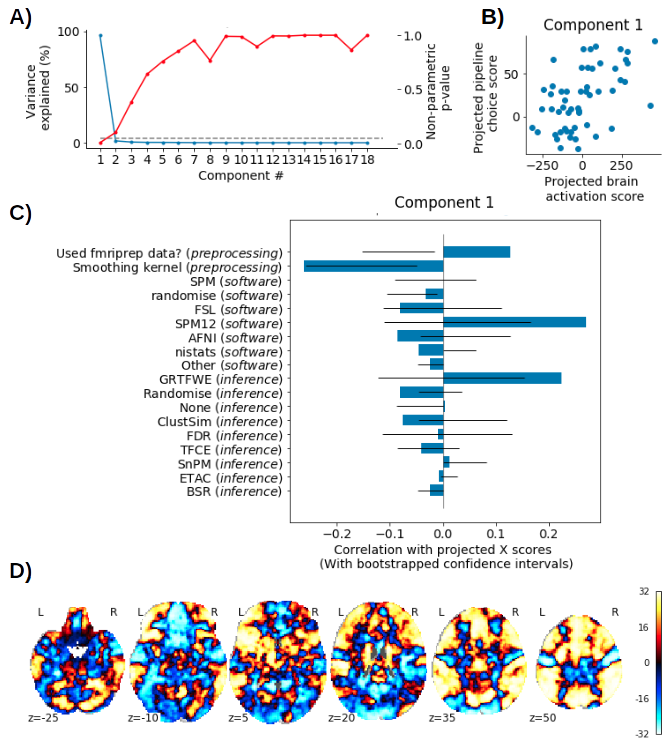
\includegraphics[width=\textwidth]{figures/results1_PLS_all.png}
	\caption{\label{fig:pls_results} PLS results. A) the variance explained and the $p$-values for each component. B) For the significant component, the correlation similarity between the projected analysis choice and brain activation scores. C) The role of each analysis-choice variable in the significant component, calculated as the correlation of the variable with its projected score, along with the bootstrapped confidence intervals to indicate the stability of its involvement.}

\end{figure}


\subsubsection{Important variables in the significant latent component}
In order to determine which analysis choices were more important in this component, we correlated the original scores with the projected scores in this new space. We then used bootstrapping to calculate confidence intervals on these correlations. In Figure \ref{fig:pls_results}C, one can see that the analysis choices whose confidence intervals do not cross zero are: whether they used the fmriprep-preprocessed data, their smoothing kernel, and whether they used randomise in FSL as their analysis software. 

In order to determine which brain areas were more important in this component, we correlated the original group-level activation maps with the projected activation scores in this space. Figure \ref{fig:pls_results} shows the bootstrap ratios for the group-level maps. While it is not in the scope of this paper to discuss the specific brain areas highlighted in this map, it is notable that the patterns are roughly symmetric, suggesting that there is meaningful structure. 

Next, we visualized one of the differences in activation across the analysis choice of whether the teams used the fmriprep-preprocessed data. This variable had the highest contribution to the component, without its confidence interval including 0. In Figure \ref{fig:fmriprep}, one can see that the results from teams using this data have a more uniform analytic range across, whereas there is notable non-uniformity in the group of teams who did their own preprocessing. 

\begin{figure}[!htb]
	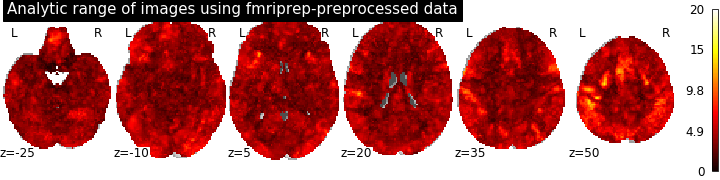
\includegraphics[width=\textwidth]
	{figures/results1B_hypo1_Analytic-range-of-images-using-fmriprep-preprocessed-data.png}
	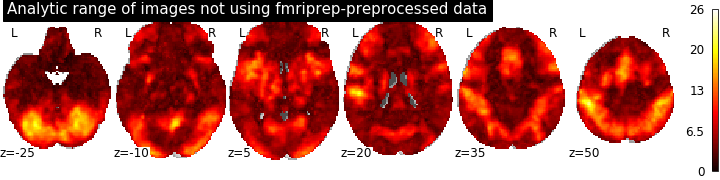
\includegraphics[width=\textwidth]
	{figures/results1B_hypo1_Analytic-range-of-images-not-using-fmriprep-preprocessed-data.png}
	\caption{\label{fig:fmriprep} Analytic range for teams who did and did not use the provided fmriprep-preprocessed data.}
\end{figure}
	

\subsection{Results II: Exploring the consensus result as a potential solution}

\subsubsection{Meta-analyses}
The results of the meta-analysis of the NARPS group-level maps can be seen in Figure \ref{fig:meta}, along with the results of the meta-analysis of the relevant literature using NeuroQuery. Based on visual inspection, the images bear little resemblance to each other.


\begin{figure}[!htb]
	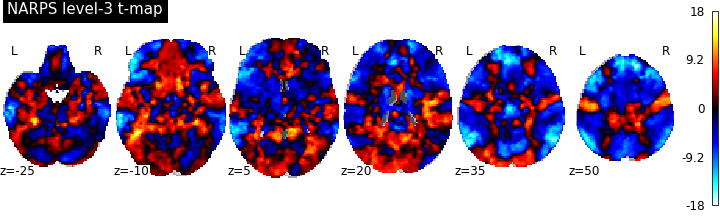
\includegraphics[width=\textwidth]
	{figures/results2A_hypo1_NARPS-level-3-t-map.png}
	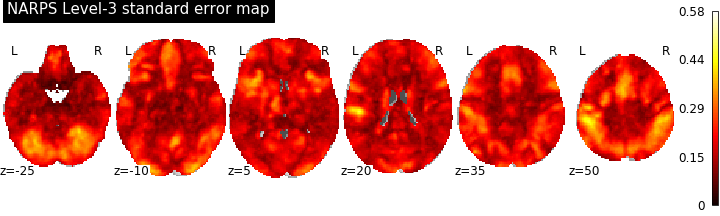
\includegraphics[width=\textwidth]
	{figures/results2A_hypo1_NARPS-Level-3-standard-error-map.png}
	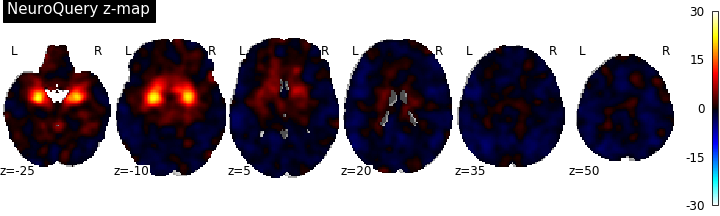
\includegraphics[width=\textwidth]
	{figures/results2A_hypo1_NeuroQuery-z-map.png}
	\caption{\label{fig:meta} Results of the meta-analysis across analysis teams. }

\end{figure}


\subsubsection{The usefulness of meta-analysis across analysis teams}

Here, we wanted to explore whether meta-analyzing group-level maps across analysis teams results in a consensus map that is more accurate than the individual group-level maps, assuming that the NeuroQuery meta-analysis of the relevant literature is the closest we can get to a ground-truth map for the cognitive task. 

In Figure \ref{fig:corr_NQ}, we see that the level-3 result of the meta-analysis on the NARPS data was weakly correlated to the NeuroQuery result, with $R_{spearman}$ = 0.085. This correlation was significant according to parametric testing, with $p$ < 0.000001. However, this testing method assumes all observations are independent, which is not the case for voxels because they are spatially autocorrelated. Using the spin test, which accounts for this autocorrelation, the $p$-value rose to 0.27. Thus, the relationship was neither large nor significant. 

In the case where this relationship were notable, we would want to determine whether it were stronger than the relationships between each individual group-level map and the NeuroQuery result. If it were stronger, this could indicate that the accuracy of results is improved when we take a meta-analysis across results with analytic variability. Despite the weak relationship between the level-3 and NeuroQuery results, in order to illustrate this type of comparison, we still calculated these comparisons between the level-2 and NeuroQuery results. 

In Figure \ref{fig:corr_NQ}, we can see that the correlation with the level-3 results was not stronger than the correlation with many of the level-2 results. Indeed, most of the level-2 results had a higher correlation. Note, however, that these comparisons were not tested for significance, and should be interpreted cautiously.

\begin{figure}[!htb]
	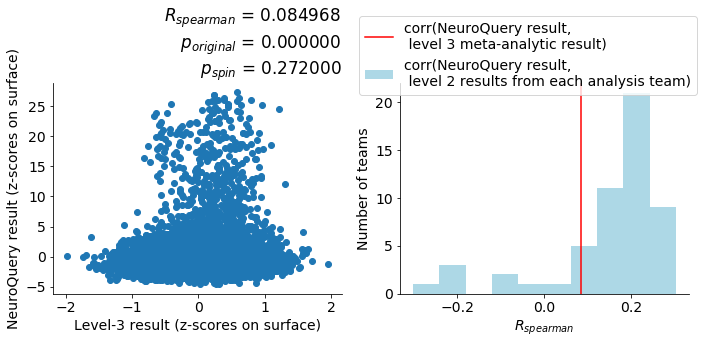
\includegraphics[width=\textwidth]
	{figures/results2B_hypo1_corr_with_NQ.png}
	\caption{\label{fig:corr_NQ} Results from the comparison with NeuroQuery to explore the usefulness of using the consensus result across analysis teams as a potential solution to the problem of analytic variability. A) Comparison of the the NeuroQuery result and the consensus map (level 3, in surface space), and B) Comparison of the relationships between the relationship between the NeuroQuery result and the consensus map (in red), and with each of the group-level maps (level 2, in light blue).}

\end{figure}

\subsection{Results III: Replication}
The replication revealed similar results, which can be seen in the Supplementary Figures section. In the replication, again the first component explained nearly all of the variance. Though the second component was significant, it explained almost no variance. There was a similar pattern for the importance of analysis choices in this component. As in the results above, the fmriprep variable was important, as well as the use of randomise. In this dataset the size of the smoothing kernel had the highest loading, but its bootstrapped confidence interval included zero, so it is not a stable result (see in Figure \ref{fig:pls_results2}C; note that the direction of correlations is irrelevant in this analysis). The distribution of bootstrap ratios over the brain, however, was visually dissimilar, though again it had some symmetry. 

\section{Discussion}
There has been concern recently over reproducibility issues in neuroimaging. These issues are partially due to analytic variability \citep{carp_plurality_2012}; results may change when different choices are made for analyzing the data \citep{carp_secret_2012}. Here, we show that, in a realistic setting where separate research teams analyze the same data, there is variety in the analysis choices and in the group-level results. PLS revealed that the analysis choices are related to the group-level results. The more important analysis choices were whether the team used the fmriprep-preprocessed data, the size of their smoothing kernel, and whether they used randomise to produce their statistical images (in FSL). In the replication data, again the fmriprep variable was important, as well as the use of randomise. A closer look at the differences in analytic range between those who do and do not use the fmriprep data reveals a spatial bias, and suggests that preprocessing is an important source of analytic variability.

We also explored the use of the consensus result across analysis teams as a way to improve the accuracy of results. To this end, we used the results of an automated meta-analysis of the relevant literature, generated using NeuroQuery, as a ground truth (or at least, a relatively closer proxy to the ground truth in this situation). The consensus result did not strongly resemble this map, and it did not have greater resemblance than the group-level maps. 

This lack of resemblance may be due to multiple reasons. It may be because the we made a poor assumption that the NeuroQuery meta-analysis could be taken as a ground truth, because the actual results from this dataset are not consistent with the past literature, or perhaps because we had a poor method for comparing these maps. Future research could further explore whether taking the consensus result is `better' in other ways, perhaps looking other measures of accuracy evaluated here, and using a better estimate of the ground truth. This may be more achievable in a study with simpler task; simpler search terms could result in a better meta-analytic result using NeuroQuery, as well enable us to use NeuroSynth \citealp{yarkoni2011large}, which only takes some single words and compound words as search terms.

Regarding further limitations, we would have preferred to replicate the results in a dataset with separate analysis teams as well as separate level-1 participants. This would improve out estimate of the generalizability of these results across new analysis teams. However, with only 55 analysis teams and many analysis choices with few teams representing that choice, we determined that it would be too difficult to split the data with instances of the same choice in each dataset.

One positive aspect of this study is that it looks at analytic variability in a more realistic setting than has been done in the past in fMRI research. However, this benefit comes with the limitation of being unable to consider or control for all possible interactions between analysis choices.  In future research, we could calculate more complex analysis-choice variables that are combinations of other variables, for example, coding which teams use both the fmriprep data as well as SPM12 by creating a new variable that is the intersection of the two original variables. Additionally, we could imitate the method of \cite{carp_secret_2012}, having one team run multiple analysis pipelines on the same data, perhaps focusing on the choices that were highlighted here as being potentially important sources of analytic variability. A related limitation is that not all analysis choices were listed; we do not know what operating systems were used, and in many cases which software versions were used, but these variables are known to impact neuroimaging results \citep{glatard_reproducibility_2015, gronenschild2012effects}.

In summary, here we find that analytic variability can contribute to differences in results, in line with previous research in less-realistic analysis settings. However, it remains unclear how best to address this issue, and whether using the consensus result across teams is an improvement over results from individual teams. These results have implications for our understanding of the stability of fMRI results across teams, and indicate that preprocessing steps may be particularly important in terms of reliability of results. There is much work to be done in this vein to improve the reliability of fMRI results. 


\section{Access to data and code}
The original participant-level data that was used by the analysis teams is publicly available on OpenNeuro.org, at \url{https://openneuro.org/datasets/ds001734/versions/1.0.4}.

The group-level images from each team will soon be made publicly available, according to \cite{botvinik-nezer_fmri_2019}.

The code used in the present study is publicly available at \url{https://github.com/koudyk/narps_meta}.

\raggedbottom

\pagebreak

\section{Supplementary Figures} \label{sec:supp_figs}
\begin{figure}[!htb]
	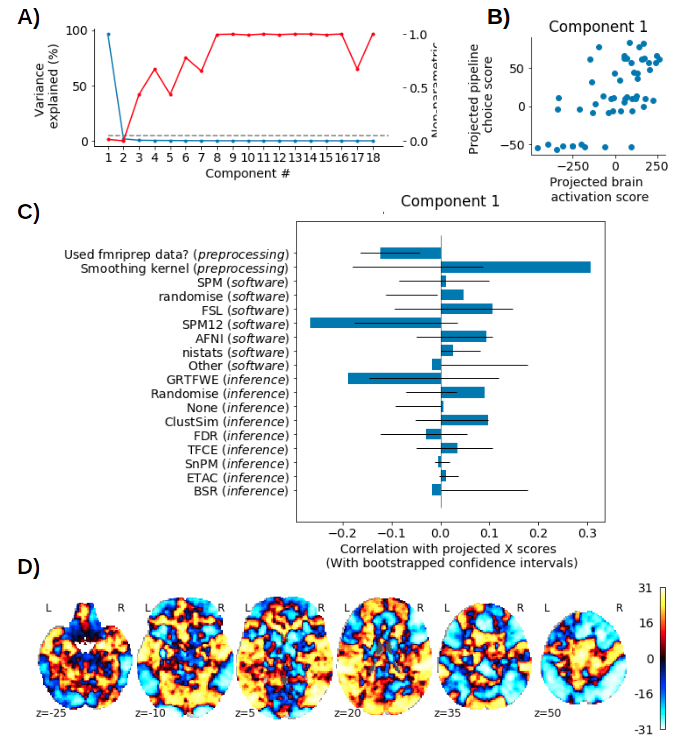
\includegraphics[width=\textwidth]{figures/results1_PLS_all_hypo2.png}
	\caption{\label{fig:pls_results2}PLS results for the replication data. A) the variance explained and the $p$-values for each component. B) For the significant component, the correlation similarity between the projected analysis choice and brain activation scores. C) The role of each analysis-choice variable in the significant component, calculated as the correlation of the variable with its projected score, along with the bootstrapped confidence intervals to indicate the stability of its involvement.}

\end{figure}

\begin{figure}[!htb]
	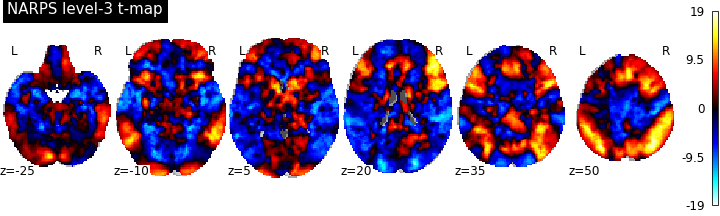
\includegraphics[width=\textwidth]
	{figures/results2A_hypo2_NARPS-level-3-t-map.png}
	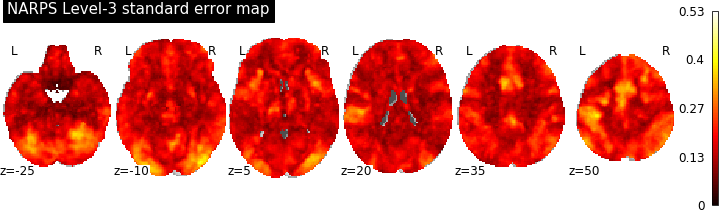
\includegraphics[width=\textwidth]
	{figures/results2A_hypo2_NARPS-Level-3-standard-error-map.png}
	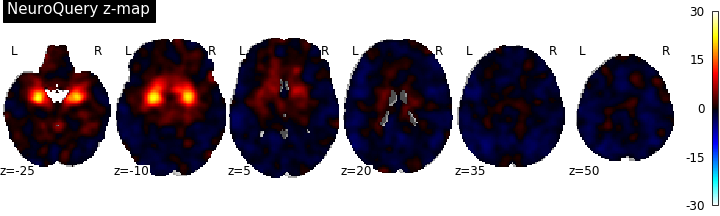
\includegraphics[width=\textwidth]
	{figures/results2A_hypo2_NeuroQuery-z-map.png}
	\caption{\label{fig:meta2} Results of the meta-analysis across analysis teams, for the replication data.}

\end{figure}
\begin{figure}[!htb]
	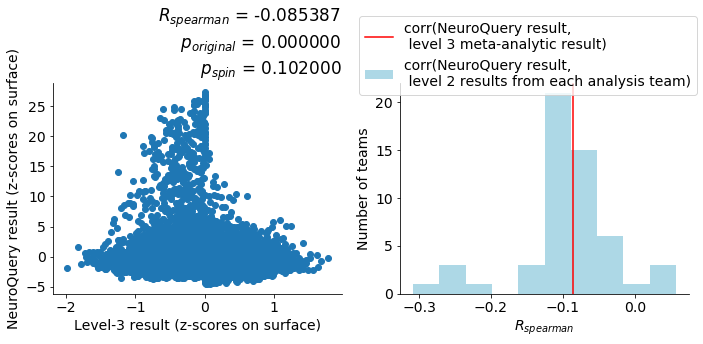
\includegraphics[width=\textwidth]
	{figures/results2B_hypo2_corr_with_NQ.png}
	\caption{\label{fig:corr_NQ2} Results from the comparison with NeuroQuery to explore the usefulness of using the consensus result across analysis teams as a potential solution to the problem of analytic variability, for the replication data. A) Comparison of the the NeuroQuery result and the consensus map (level 3, in surface space), and B) Comparison of the relationships between the relationship between the NeuroQuery result and the consensus map (in red), and with each of the group-level maps (level 2, in light blue).}

\end{figure}







\clearpage
\bibliography{references}
\bibliographystyle{plain}




\end{document}

%
% Please see the package documentation for more information
% on the APA6 document class:
%
% http://www.ctan.org/pkg/apa6
%